% Created by tikzDevice version 0.10.1.2 on 2018-03-05 22:39:51
% !TEX encoding = UTF-8 Unicode
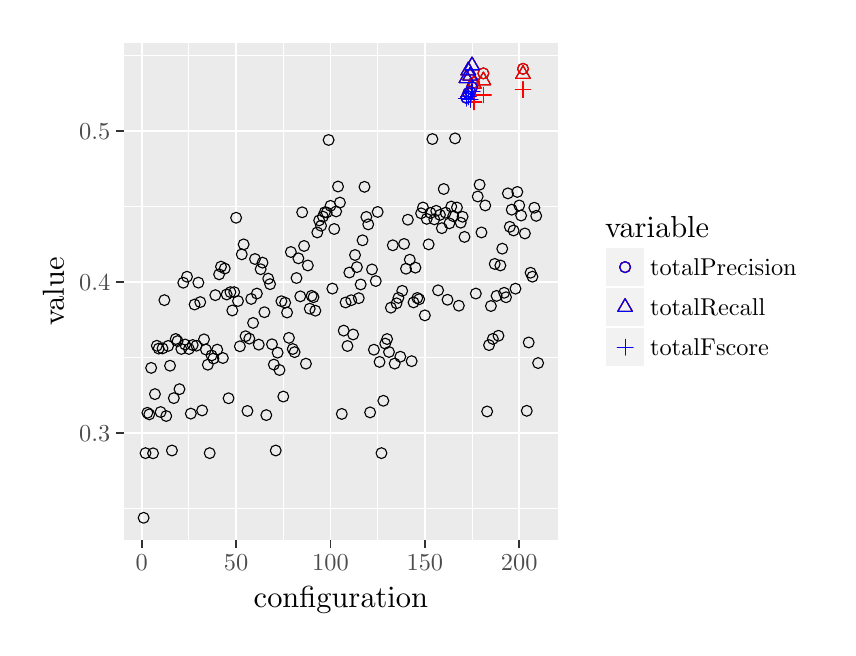
\begin{tikzpicture}[x=1pt,y=1pt]
\definecolor{fillColor}{RGB}{255,255,255}
\path[use as bounding box,fill=fillColor,fill opacity=0.00] (0,0) rectangle (289.08,216.81);
\begin{scope}
\path[clip] (  0.00,  0.00) rectangle (289.08,216.81);
\definecolor{drawColor}{RGB}{255,255,255}
\definecolor{fillColor}{RGB}{255,255,255}

\path[draw=drawColor,line width= 0.6pt,line join=round,line cap=round,fill=fillColor] (  0.00,  0.00) rectangle (289.08,216.81);
\end{scope}
\begin{scope}
\path[clip] ( 34.77, 31.53) rectangle (191.57,211.31);
\definecolor{fillColor}{gray}{0.92}

\path[fill=fillColor] ( 34.77, 31.53) rectangle (191.57,211.31);
\definecolor{drawColor}{RGB}{255,255,255}

\path[draw=drawColor,line width= 0.3pt,line join=round] ( 34.77, 43.14) --
	(191.57, 43.14);

\path[draw=drawColor,line width= 0.3pt,line join=round] ( 34.77, 97.66) --
	(191.57, 97.66);

\path[draw=drawColor,line width= 0.3pt,line join=round] ( 34.77,152.19) --
	(191.57,152.19);

\path[draw=drawColor,line width= 0.3pt,line join=round] ( 34.77,206.71) --
	(191.57,206.71);

\path[draw=drawColor,line width= 0.3pt,line join=round] ( 58.26, 31.53) --
	( 58.26,211.31);

\path[draw=drawColor,line width= 0.3pt,line join=round] ( 92.37, 31.53) --
	( 92.37,211.31);

\path[draw=drawColor,line width= 0.3pt,line join=round] (126.47, 31.53) --
	(126.47,211.31);

\path[draw=drawColor,line width= 0.3pt,line join=round] (160.57, 31.53) --
	(160.57,211.31);

\path[draw=drawColor,line width= 0.6pt,line join=round] ( 34.77, 70.40) --
	(191.57, 70.40);

\path[draw=drawColor,line width= 0.6pt,line join=round] ( 34.77,124.92) --
	(191.57,124.92);

\path[draw=drawColor,line width= 0.6pt,line join=round] ( 34.77,179.45) --
	(191.57,179.45);

\path[draw=drawColor,line width= 0.6pt,line join=round] ( 41.21, 31.53) --
	( 41.21,211.31);

\path[draw=drawColor,line width= 0.6pt,line join=round] ( 75.32, 31.53) --
	( 75.32,211.31);

\path[draw=drawColor,line width= 0.6pt,line join=round] (109.42, 31.53) --
	(109.42,211.31);

\path[draw=drawColor,line width= 0.6pt,line join=round] (143.52, 31.53) --
	(143.52,211.31);

\path[draw=drawColor,line width= 0.6pt,line join=round] (177.63, 31.53) --
	(177.63,211.31);
\definecolor{drawColor}{RGB}{0,0,0}

\path[draw=drawColor,line width= 0.4pt,line join=round,line cap=round] ( 41.90, 39.70) circle (  1.96);

\path[draw=drawColor,line width= 0.4pt,line join=round,line cap=round] ( 42.58, 63.07) circle (  1.96);

\path[draw=drawColor,line width= 0.4pt,line join=round,line cap=round] ( 43.26, 77.65) circle (  1.96);

\path[draw=drawColor,line width= 0.4pt,line join=round,line cap=round] ( 43.94, 77.08) circle (  1.96);

\path[draw=drawColor,line width= 0.4pt,line join=round,line cap=round] ( 44.62, 93.87) circle (  1.96);

\path[draw=drawColor,line width= 0.4pt,line join=round,line cap=round] ( 45.31, 63.01) circle (  1.96);

\path[draw=drawColor,line width= 0.4pt,line join=round,line cap=round] ( 45.99, 84.39) circle (  1.96);

\path[draw=drawColor,line width= 0.4pt,line join=round,line cap=round] ( 46.67,101.86) circle (  1.96);

\path[draw=drawColor,line width= 0.4pt,line join=round,line cap=round] ( 47.35,100.85) circle (  1.96);

\path[draw=drawColor,line width= 0.4pt,line join=round,line cap=round] ( 48.03, 77.92) circle (  1.96);

\path[draw=drawColor,line width= 0.4pt,line join=round,line cap=round] ( 48.72,100.91) circle (  1.96);

\path[draw=drawColor,line width= 0.4pt,line join=round,line cap=round] ( 49.40,118.35) circle (  1.96);

\path[draw=drawColor,line width= 0.4pt,line join=round,line cap=round] ( 50.08, 76.48) circle (  1.96);

\path[draw=drawColor,line width= 0.4pt,line join=round,line cap=round] ( 50.76,101.81) circle (  1.96);

\path[draw=drawColor,line width= 0.4pt,line join=round,line cap=round] ( 51.44, 94.66) circle (  1.96);

\path[draw=drawColor,line width= 0.4pt,line join=round,line cap=round] ( 52.13, 64.02) circle (  1.96);

\path[draw=drawColor,line width= 0.4pt,line join=round,line cap=round] ( 52.81, 82.94) circle (  1.96);

\path[draw=drawColor,line width= 0.4pt,line join=round,line cap=round] ( 53.49,104.31) circle (  1.96);

\path[draw=drawColor,line width= 0.4pt,line join=round,line cap=round] ( 54.17,103.55) circle (  1.96);

\path[draw=drawColor,line width= 0.4pt,line join=round,line cap=round] ( 54.85, 86.18) circle (  1.96);

\path[draw=drawColor,line width= 0.4pt,line join=round,line cap=round] ( 55.54,100.72) circle (  1.96);

\path[draw=drawColor,line width= 0.4pt,line join=round,line cap=round] ( 56.22,124.65) circle (  1.96);

\path[draw=drawColor,line width= 0.4pt,line join=round,line cap=round] ( 56.90,102.32) circle (  1.96);

\path[draw=drawColor,line width= 0.4pt,line join=round,line cap=round] ( 57.58,126.81) circle (  1.96);

\path[draw=drawColor,line width= 0.4pt,line join=round,line cap=round] ( 58.26,100.72) circle (  1.96);

\path[draw=drawColor,line width= 0.4pt,line join=round,line cap=round] ( 58.95, 77.35) circle (  1.96);

\path[draw=drawColor,line width= 0.4pt,line join=round,line cap=round] ( 59.63,102.13) circle (  1.96);

\path[draw=drawColor,line width= 0.4pt,line join=round,line cap=round] ( 60.31,116.77) circle (  1.96);

\path[draw=drawColor,line width= 0.4pt,line join=round,line cap=round] ( 60.99,101.89) circle (  1.96);

\path[draw=drawColor,line width= 0.4pt,line join=round,line cap=round] ( 61.68,124.68) circle (  1.96);

\path[draw=drawColor,line width= 0.4pt,line join=round,line cap=round] ( 62.36,117.65) circle (  1.96);

\path[draw=drawColor,line width= 0.4pt,line join=round,line cap=round] ( 63.04, 78.50) circle (  1.96);

\path[draw=drawColor,line width= 0.4pt,line join=round,line cap=round] ( 63.72,104.18) circle (  1.96);

\path[draw=drawColor,line width= 0.4pt,line join=round,line cap=round] ( 64.40,100.50) circle (  1.96);

\path[draw=drawColor,line width= 0.4pt,line join=round,line cap=round] ( 65.09, 95.02) circle (  1.96);

\path[draw=drawColor,line width= 0.4pt,line join=round,line cap=round] ( 65.77, 63.07) circle (  1.96);

\path[draw=drawColor,line width= 0.4pt,line join=round,line cap=round] ( 66.45, 98.37) circle (  1.96);

\path[draw=drawColor,line width= 0.4pt,line join=round,line cap=round] ( 67.13, 97.25) circle (  1.96);

\path[draw=drawColor,line width= 0.4pt,line join=round,line cap=round] ( 67.81,120.15) circle (  1.96);

\path[draw=drawColor,line width= 0.4pt,line join=round,line cap=round] ( 68.50,100.47) circle (  1.96);

\path[draw=drawColor,line width= 0.4pt,line join=round,line cap=round] ( 69.18,127.68) circle (  1.96);

\path[draw=drawColor,line width= 0.4pt,line join=round,line cap=round] ( 69.86,130.46) circle (  1.96);

\path[draw=drawColor,line width= 0.4pt,line join=round,line cap=round] ( 70.54, 97.44) circle (  1.96);

\path[draw=drawColor,line width= 0.4pt,line join=round,line cap=round] ( 71.22,129.78) circle (  1.96);

\path[draw=drawColor,line width= 0.4pt,line join=round,line cap=round] ( 71.91,120.40) circle (  1.96);

\path[draw=drawColor,line width= 0.4pt,line join=round,line cap=round] ( 72.59, 82.89) circle (  1.96);

\path[draw=drawColor,line width= 0.4pt,line join=round,line cap=round] ( 73.27,121.24) circle (  1.96);

\path[draw=drawColor,line width= 0.4pt,line join=round,line cap=round] ( 73.95,114.62) circle (  1.96);

\path[draw=drawColor,line width= 0.4pt,line join=round,line cap=round] ( 74.63,121.24) circle (  1.96);

\path[draw=drawColor,line width= 0.4pt,line join=round,line cap=round] ( 75.32,148.12) circle (  1.96);

\path[draw=drawColor,line width= 0.4pt,line join=round,line cap=round] ( 76.00,118.03) circle (  1.96);

\path[draw=drawColor,line width= 0.4pt,line join=round,line cap=round] ( 76.68,101.67) circle (  1.96);

\path[draw=drawColor,line width= 0.4pt,line join=round,line cap=round] ( 77.36,134.90) circle (  1.96);

\path[draw=drawColor,line width= 0.4pt,line join=round,line cap=round] ( 78.04,138.50) circle (  1.96);

\path[draw=drawColor,line width= 0.4pt,line join=round,line cap=round] ( 78.73,105.32) circle (  1.96);

\path[draw=drawColor,line width= 0.4pt,line join=round,line cap=round] ( 79.41, 78.31) circle (  1.96);

\path[draw=drawColor,line width= 0.4pt,line join=round,line cap=round] ( 80.09,104.45) circle (  1.96);

\path[draw=drawColor,line width= 0.4pt,line join=round,line cap=round] ( 80.77,118.79) circle (  1.96);

\path[draw=drawColor,line width= 0.4pt,line join=round,line cap=round] ( 81.45,110.12) circle (  1.96);

\path[draw=drawColor,line width= 0.4pt,line join=round,line cap=round] ( 82.14,133.21) circle (  1.96);

\path[draw=drawColor,line width= 0.4pt,line join=round,line cap=round] ( 82.82,120.73) circle (  1.96);

\path[draw=drawColor,line width= 0.4pt,line join=round,line cap=round] ( 83.50,102.27) circle (  1.96);

\path[draw=drawColor,line width= 0.4pt,line join=round,line cap=round] ( 84.18,129.53) circle (  1.96);

\path[draw=drawColor,line width= 0.4pt,line join=round,line cap=round] ( 84.87,131.90) circle (  1.96);

\path[draw=drawColor,line width= 0.4pt,line join=round,line cap=round] ( 85.55,113.99) circle (  1.96);

\path[draw=drawColor,line width= 0.4pt,line join=round,line cap=round] ( 86.23, 76.81) circle (  1.96);

\path[draw=drawColor,line width= 0.4pt,line join=round,line cap=round] ( 86.91,126.12) circle (  1.96);

\path[draw=drawColor,line width= 0.4pt,line join=round,line cap=round] ( 87.59,124.13) circle (  1.96);

\path[draw=drawColor,line width= 0.4pt,line join=round,line cap=round] ( 88.28,102.41) circle (  1.96);

\path[draw=drawColor,line width= 0.4pt,line join=round,line cap=round] ( 88.96, 95.07) circle (  1.96);

\path[draw=drawColor,line width= 0.4pt,line join=round,line cap=round] ( 89.64, 64.02) circle (  1.96);

\path[draw=drawColor,line width= 0.4pt,line join=round,line cap=round] ( 90.32, 99.38) circle (  1.96);

\path[draw=drawColor,line width= 0.4pt,line join=round,line cap=round] ( 91.00, 93.11) circle (  1.96);

\path[draw=drawColor,line width= 0.4pt,line join=round,line cap=round] ( 91.69,117.97) circle (  1.96);

\path[draw=drawColor,line width= 0.4pt,line join=round,line cap=round] ( 92.37, 83.51) circle (  1.96);

\path[draw=drawColor,line width= 0.4pt,line join=round,line cap=round] ( 93.05,117.43) circle (  1.96);

\path[draw=drawColor,line width= 0.4pt,line join=round,line cap=round] ( 93.73,113.88) circle (  1.96);

\path[draw=drawColor,line width= 0.4pt,line join=round,line cap=round] ( 94.41,104.72) circle (  1.96);

\path[draw=drawColor,line width= 0.4pt,line join=round,line cap=round] ( 95.10,135.75) circle (  1.96);

\path[draw=drawColor,line width= 0.4pt,line join=round,line cap=round] ( 95.78,100.69) circle (  1.96);

\path[draw=drawColor,line width= 0.4pt,line join=round,line cap=round] ( 96.46, 99.57) circle (  1.96);

\path[draw=drawColor,line width= 0.4pt,line join=round,line cap=round] ( 97.14,126.34) circle (  1.96);

\path[draw=drawColor,line width= 0.4pt,line join=round,line cap=round] ( 97.82,133.46) circle (  1.96);

\path[draw=drawColor,line width= 0.4pt,line join=round,line cap=round] ( 98.51,119.72) circle (  1.96);

\path[draw=drawColor,line width= 0.4pt,line join=round,line cap=round] ( 99.19,150.09) circle (  1.96);

\path[draw=drawColor,line width= 0.4pt,line join=round,line cap=round] ( 99.87,137.93) circle (  1.96);

\path[draw=drawColor,line width= 0.4pt,line join=round,line cap=round] (100.55, 95.40) circle (  1.96);

\path[draw=drawColor,line width= 0.4pt,line join=round,line cap=round] (101.23,130.89) circle (  1.96);

\path[draw=drawColor,line width= 0.4pt,line join=round,line cap=round] (101.92,115.27) circle (  1.96);

\path[draw=drawColor,line width= 0.4pt,line join=round,line cap=round] (102.60,119.91) circle (  1.96);

\path[draw=drawColor,line width= 0.4pt,line join=round,line cap=round] (103.28,119.42) circle (  1.96);

\path[draw=drawColor,line width= 0.4pt,line join=round,line cap=round] (103.96,114.54) circle (  1.96);

\path[draw=drawColor,line width= 0.4pt,line join=round,line cap=round] (104.65,142.81) circle (  1.96);

\path[draw=drawColor,line width= 0.4pt,line join=round,line cap=round] (105.33,147.17) circle (  1.96);

\path[draw=drawColor,line width= 0.4pt,line join=round,line cap=round] (106.01,145.23) circle (  1.96);

\path[draw=drawColor,line width= 0.4pt,line join=round,line cap=round] (106.69,148.53) circle (  1.96);

\path[draw=drawColor,line width= 0.4pt,line join=round,line cap=round] (107.37,150.11) circle (  1.96);

\path[draw=drawColor,line width= 0.4pt,line join=round,line cap=round] (108.06,150.03) circle (  1.96);

\path[draw=drawColor,line width= 0.4pt,line join=round,line cap=round] (108.74,176.23) circle (  1.96);

\path[draw=drawColor,line width= 0.4pt,line join=round,line cap=round] (109.42,152.43) circle (  1.96);

\path[draw=drawColor,line width= 0.4pt,line join=round,line cap=round] (110.10,122.53) circle (  1.96);

\path[draw=drawColor,line width= 0.4pt,line join=round,line cap=round] (110.78,144.06) circle (  1.96);

\path[draw=drawColor,line width= 0.4pt,line join=round,line cap=round] (111.47,150.41) circle (  1.96);

\path[draw=drawColor,line width= 0.4pt,line join=round,line cap=round] (112.15,159.41) circle (  1.96);

\path[draw=drawColor,line width= 0.4pt,line join=round,line cap=round] (112.83,153.60) circle (  1.96);

\path[draw=drawColor,line width= 0.4pt,line join=round,line cap=round] (113.51, 77.24) circle (  1.96);

\path[draw=drawColor,line width= 0.4pt,line join=round,line cap=round] (114.19,107.34) circle (  1.96);

\path[draw=drawColor,line width= 0.4pt,line join=round,line cap=round] (114.88,117.51) circle (  1.96);

\path[draw=drawColor,line width= 0.4pt,line join=round,line cap=round] (115.56,101.78) circle (  1.96);

\path[draw=drawColor,line width= 0.4pt,line join=round,line cap=round] (116.24,128.33) circle (  1.96);

\path[draw=drawColor,line width= 0.4pt,line join=round,line cap=round] (116.92,118.33) circle (  1.96);

\path[draw=drawColor,line width= 0.4pt,line join=round,line cap=round] (117.60,105.95) circle (  1.96);

\path[draw=drawColor,line width= 0.4pt,line join=round,line cap=round] (118.29,134.66) circle (  1.96);

\path[draw=drawColor,line width= 0.4pt,line join=round,line cap=round] (118.97,130.29) circle (  1.96);

\path[draw=drawColor,line width= 0.4pt,line join=round,line cap=round] (119.65,119.06) circle (  1.96);

\path[draw=drawColor,line width= 0.4pt,line join=round,line cap=round] (120.33,124.02) circle (  1.96);

\path[draw=drawColor,line width= 0.4pt,line join=round,line cap=round] (121.01,139.97) circle (  1.96);

\path[draw=drawColor,line width= 0.4pt,line join=round,line cap=round] (121.70,159.30) circle (  1.96);

\path[draw=drawColor,line width= 0.4pt,line join=round,line cap=round] (122.38,148.42) circle (  1.96);

\path[draw=drawColor,line width= 0.4pt,line join=round,line cap=round] (123.06,145.73) circle (  1.96);

\path[draw=drawColor,line width= 0.4pt,line join=round,line cap=round] (123.74, 77.79) circle (  1.96);

\path[draw=drawColor,line width= 0.4pt,line join=round,line cap=round] (124.42,129.45) circle (  1.96);

\path[draw=drawColor,line width= 0.4pt,line join=round,line cap=round] (125.11,100.44) circle (  1.96);

\path[draw=drawColor,line width= 0.4pt,line join=round,line cap=round] (125.79,125.25) circle (  1.96);

\path[draw=drawColor,line width= 0.4pt,line join=round,line cap=round] (126.47,150.22) circle (  1.96);

\path[draw=drawColor,line width= 0.4pt,line join=round,line cap=round] (127.15, 96.03) circle (  1.96);

\path[draw=drawColor,line width= 0.4pt,line join=round,line cap=round] (127.84, 63.07) circle (  1.96);

\path[draw=drawColor,line width= 0.4pt,line join=round,line cap=round] (128.52, 81.99) circle (  1.96);

\path[draw=drawColor,line width= 0.4pt,line join=round,line cap=round] (129.20,102.65) circle (  1.96);

\path[draw=drawColor,line width= 0.4pt,line join=round,line cap=round] (129.88,104.29) circle (  1.96);

\path[draw=drawColor,line width= 0.4pt,line join=round,line cap=round] (130.56, 99.62) circle (  1.96);

\path[draw=drawColor,line width= 0.4pt,line join=round,line cap=round] (131.25,115.63) circle (  1.96);

\path[draw=drawColor,line width= 0.4pt,line join=round,line cap=round] (131.93,138.17) circle (  1.96);

\path[draw=drawColor,line width= 0.4pt,line join=round,line cap=round] (132.61, 95.43) circle (  1.96);

\path[draw=drawColor,line width= 0.4pt,line join=round,line cap=round] (133.29,117.21) circle (  1.96);

\path[draw=drawColor,line width= 0.4pt,line join=round,line cap=round] (133.97,119.17) circle (  1.96);

\path[draw=drawColor,line width= 0.4pt,line join=round,line cap=round] (134.66, 97.91) circle (  1.96);

\path[draw=drawColor,line width= 0.4pt,line join=round,line cap=round] (135.34,121.71) circle (  1.96);

\path[draw=drawColor,line width= 0.4pt,line join=round,line cap=round] (136.02,138.66) circle (  1.96);

\path[draw=drawColor,line width= 0.4pt,line join=round,line cap=round] (136.70,129.70) circle (  1.96);

\path[draw=drawColor,line width= 0.4pt,line join=round,line cap=round] (137.38,147.42) circle (  1.96);

\path[draw=drawColor,line width= 0.4pt,line join=round,line cap=round] (138.07,132.97) circle (  1.96);

\path[draw=drawColor,line width= 0.4pt,line join=round,line cap=round] (138.75, 96.30) circle (  1.96);

\path[draw=drawColor,line width= 0.4pt,line join=round,line cap=round] (139.43,117.54) circle (  1.96);

\path[draw=drawColor,line width= 0.4pt,line join=round,line cap=round] (140.11,130.10) circle (  1.96);

\path[draw=drawColor,line width= 0.4pt,line join=round,line cap=round] (140.79,119.14) circle (  1.96);

\path[draw=drawColor,line width= 0.4pt,line join=round,line cap=round] (141.48,118.68) circle (  1.96);

\path[draw=drawColor,line width= 0.4pt,line join=round,line cap=round] (142.16,149.73) circle (  1.96);

\path[draw=drawColor,line width= 0.4pt,line join=round,line cap=round] (142.84,151.83) circle (  1.96);

\path[draw=drawColor,line width= 0.4pt,line join=round,line cap=round] (143.52,112.85) circle (  1.96);

\path[draw=drawColor,line width= 0.4pt,line join=round,line cap=round] (144.20,147.72) circle (  1.96);

\path[draw=drawColor,line width= 0.4pt,line join=round,line cap=round] (144.89,138.50) circle (  1.96);

\path[draw=drawColor,line width= 0.4pt,line join=round,line cap=round] (145.57,149.87) circle (  1.96);

\path[draw=drawColor,line width= 0.4pt,line join=round,line cap=round] (146.25,176.56) circle (  1.96);

\path[draw=drawColor,line width= 0.4pt,line join=round,line cap=round] (146.93,147.55) circle (  1.96);

\path[draw=drawColor,line width= 0.4pt,line join=round,line cap=round] (147.62,150.63) circle (  1.96);

\path[draw=drawColor,line width= 0.4pt,line join=round,line cap=round] (148.30,121.90) circle (  1.96);

\path[draw=drawColor,line width= 0.4pt,line join=round,line cap=round] (148.98,149.16) circle (  1.96);

\path[draw=drawColor,line width= 0.4pt,line join=round,line cap=round] (149.66,144.36) circle (  1.96);

\path[draw=drawColor,line width= 0.4pt,line join=round,line cap=round] (150.34,158.51) circle (  1.96);

\path[draw=drawColor,line width= 0.4pt,line join=round,line cap=round] (151.03,149.95) circle (  1.96);

\path[draw=drawColor,line width= 0.4pt,line join=round,line cap=round] (151.71,118.49) circle (  1.96);

\path[draw=drawColor,line width= 0.4pt,line join=round,line cap=round] (152.39,146.11) circle (  1.96);

\path[draw=drawColor,line width= 0.4pt,line join=round,line cap=round] (153.07,152.16) circle (  1.96);

\path[draw=drawColor,line width= 0.4pt,line join=round,line cap=round] (153.75,148.72) circle (  1.96);

\path[draw=drawColor,line width= 0.4pt,line join=round,line cap=round] (154.44,176.80) circle (  1.96);

\path[draw=drawColor,line width= 0.4pt,line join=round,line cap=round] (155.12,151.83) circle (  1.96);

\path[draw=drawColor,line width= 0.4pt,line join=round,line cap=round] (155.80,116.34) circle (  1.96);

\path[draw=drawColor,line width= 0.4pt,line join=round,line cap=round] (156.48,146.33) circle (  1.96);

\path[draw=drawColor,line width= 0.4pt,line join=round,line cap=round] (157.16,148.48) circle (  1.96);

\path[draw=drawColor,line width= 0.4pt,line join=round,line cap=round] (157.85,141.20) circle (  1.96);

\path[draw=drawColor,line width= 0.4pt,line join=round,line cap=round] (158.53,191.47) circle (  1.96);

\path[draw=drawColor,line width= 0.4pt,line join=round,line cap=round] (159.21,193.13) circle (  1.96);

\path[draw=drawColor,line width= 0.4pt,line join=round,line cap=round] (159.89,193.63) circle (  1.96);

\path[draw=drawColor,line width= 0.4pt,line join=round,line cap=round] (160.57,195.34) circle (  1.96);

\path[draw=drawColor,line width= 0.4pt,line join=round,line cap=round] (161.26,196.98) circle (  1.96);

\path[draw=drawColor,line width= 0.4pt,line join=round,line cap=round] (161.94,120.73) circle (  1.96);

\path[draw=drawColor,line width= 0.4pt,line join=round,line cap=round] (162.62,155.81) circle (  1.96);

\path[draw=drawColor,line width= 0.4pt,line join=round,line cap=round] (163.30,160.07) circle (  1.96);

\path[draw=drawColor,line width= 0.4pt,line join=round,line cap=round] (163.98,142.81) circle (  1.96);

\path[draw=drawColor,line width= 0.4pt,line join=round,line cap=round] (164.67,200.30) circle (  1.96);

\path[draw=drawColor,line width= 0.4pt,line join=round,line cap=round] (165.35,152.57) circle (  1.96);

\path[draw=drawColor,line width= 0.4pt,line join=round,line cap=round] (166.03, 78.12) circle (  1.96);

\path[draw=drawColor,line width= 0.4pt,line join=round,line cap=round] (166.71,102.11) circle (  1.96);

\path[draw=drawColor,line width= 0.4pt,line join=round,line cap=round] (167.39,116.23) circle (  1.96);

\path[draw=drawColor,line width= 0.4pt,line join=round,line cap=round] (168.08,104.34) circle (  1.96);

\path[draw=drawColor,line width= 0.4pt,line join=round,line cap=round] (168.76,131.44) circle (  1.96);

\path[draw=drawColor,line width= 0.4pt,line join=round,line cap=round] (169.44,119.88) circle (  1.96);

\path[draw=drawColor,line width= 0.4pt,line join=round,line cap=round] (170.12,105.49) circle (  1.96);

\path[draw=drawColor,line width= 0.4pt,line join=round,line cap=round] (170.81,130.89) circle (  1.96);

\path[draw=drawColor,line width= 0.4pt,line join=round,line cap=round] (171.49,136.95) circle (  1.96);

\path[draw=drawColor,line width= 0.4pt,line join=round,line cap=round] (172.17,121.00) circle (  1.96);

\path[draw=drawColor,line width= 0.4pt,line join=round,line cap=round] (172.85,119.39) circle (  1.96);

\path[draw=drawColor,line width= 0.4pt,line join=round,line cap=round] (173.53,156.93) circle (  1.96);

\path[draw=drawColor,line width= 0.4pt,line join=round,line cap=round] (174.22,144.85) circle (  1.96);

\path[draw=drawColor,line width= 0.4pt,line join=round,line cap=round] (174.90,151.04) circle (  1.96);

\path[draw=drawColor,line width= 0.4pt,line join=round,line cap=round] (175.58,143.52) circle (  1.96);

\path[draw=drawColor,line width= 0.4pt,line join=round,line cap=round] (176.26,122.50) circle (  1.96);

\path[draw=drawColor,line width= 0.4pt,line join=round,line cap=round] (176.94,157.45) circle (  1.96);

\path[draw=drawColor,line width= 0.4pt,line join=round,line cap=round] (177.63,152.57) circle (  1.96);

\path[draw=drawColor,line width= 0.4pt,line join=round,line cap=round] (178.31,148.92) circle (  1.96);

\path[draw=drawColor,line width= 0.4pt,line join=round,line cap=round] (178.99,201.94) circle (  1.96);

\path[draw=drawColor,line width= 0.4pt,line join=round,line cap=round] (179.67,142.45) circle (  1.96);

\path[draw=drawColor,line width= 0.4pt,line join=round,line cap=round] (180.35, 78.36) circle (  1.96);

\path[draw=drawColor,line width= 0.4pt,line join=round,line cap=round] (181.04,103.06) circle (  1.96);

\path[draw=drawColor,line width= 0.4pt,line join=round,line cap=round] (181.72,128.25) circle (  1.96);

\path[draw=drawColor,line width= 0.4pt,line join=round,line cap=round] (182.40,126.83) circle (  1.96);

\path[draw=drawColor,line width= 0.4pt,line join=round,line cap=round] (183.08,151.75) circle (  1.96);

\path[draw=drawColor,line width= 0.4pt,line join=round,line cap=round] (183.76,148.81) circle (  1.96);

\path[draw=drawColor,line width= 0.4pt,line join=round,line cap=round] (184.45, 95.62) circle (  1.96);

\path[draw=drawColor,line width= 0.4pt,line join=round,line cap=round] (158.53,201.52) --
	(161.17,196.95) --
	(155.89,196.95) --
	(158.53,201.52);

\path[draw=drawColor,line width= 0.4pt,line join=round,line cap=round] (159.21,204.34) --
	(161.85,199.76) --
	(156.57,199.76) --
	(159.21,204.34);

\path[draw=drawColor,line width= 0.4pt,line join=round,line cap=round] (159.89,202.43) --
	(162.53,197.86) --
	(157.25,197.86) --
	(159.89,202.43);

\path[draw=drawColor,line width= 0.4pt,line join=round,line cap=round] (160.57,206.19) --
	(163.22,201.61) --
	(157.93,201.61) --
	(160.57,206.19);

\path[draw=drawColor,line width= 0.4pt,line join=round,line cap=round] (161.26,199.50) --
	(163.90,194.92) --
	(158.61,194.92) --
	(161.26,199.50);

\path[draw=drawColor,line width= 0.4pt,line join=round,line cap=round] (164.67,200.77) --
	(167.31,196.19) --
	(162.02,196.19) --
	(164.67,200.77);

\path[draw=drawColor,line width= 0.4pt,line join=round,line cap=round] (178.99,203.07) --
	(181.63,198.49) --
	(176.35,198.49) --
	(178.99,203.07);

\path[draw=drawColor,line width= 0.4pt,line join=round,line cap=round] (155.75,191.33) -- (161.30,191.33);

\path[draw=drawColor,line width= 0.4pt,line join=round,line cap=round] (158.53,188.56) -- (158.53,194.11);

\path[draw=drawColor,line width= 0.4pt,line join=round,line cap=round] (156.44,191.80) -- (161.99,191.80);

\path[draw=drawColor,line width= 0.4pt,line join=round,line cap=round] (159.21,189.02) -- (159.21,194.57);

\path[draw=drawColor,line width= 0.4pt,line join=round,line cap=round] (157.12,190.90) -- (162.67,190.90);

\path[draw=drawColor,line width= 0.4pt,line join=round,line cap=round] (159.89,188.13) -- (159.89,193.68);

\path[draw=drawColor,line width= 0.4pt,line join=round,line cap=round] (157.80,193.70) -- (163.35,193.70);

\path[draw=drawColor,line width= 0.4pt,line join=round,line cap=round] (160.57,190.93) -- (160.57,196.48);

\path[draw=drawColor,line width= 0.4pt,line join=round,line cap=round] (158.48,189.95) -- (164.03,189.95);

\path[draw=drawColor,line width= 0.4pt,line join=round,line cap=round] (161.26,187.17) -- (161.26,192.72);

\path[draw=drawColor,line width= 0.4pt,line join=round,line cap=round] (161.89,192.49) -- (167.44,192.49);

\path[draw=drawColor,line width= 0.4pt,line join=round,line cap=round] (164.67,189.71) -- (164.67,195.26);

\path[draw=drawColor,line width= 0.4pt,line join=round,line cap=round] (176.22,194.45) -- (181.76,194.45);

\path[draw=drawColor,line width= 0.4pt,line join=round,line cap=round] (178.99,191.67) -- (178.99,197.22);
\definecolor{drawColor}{RGB}{255,0,0}

\path[draw=drawColor,line width= 0.4pt,line join=round,line cap=round] (158.53,191.47) circle (  1.96);

\path[draw=drawColor,line width= 0.4pt,line join=round,line cap=round] (159.21,193.13) circle (  1.96);

\path[draw=drawColor,line width= 0.4pt,line join=round,line cap=round] (159.89,193.63) circle (  1.96);

\path[draw=drawColor,line width= 0.4pt,line join=round,line cap=round] (160.57,195.34) circle (  1.96);

\path[draw=drawColor,line width= 0.4pt,line join=round,line cap=round] (161.26,196.98) circle (  1.96);

\path[draw=drawColor,line width= 0.4pt,line join=round,line cap=round] (164.67,200.30) circle (  1.96);

\path[draw=drawColor,line width= 0.4pt,line join=round,line cap=round] (178.99,201.94) circle (  1.96);

\path[draw=drawColor,line width= 0.4pt,line join=round,line cap=round] (158.53,201.52) --
	(161.17,196.95) --
	(155.89,196.95) --
	(158.53,201.52);

\path[draw=drawColor,line width= 0.4pt,line join=round,line cap=round] (159.21,204.34) --
	(161.85,199.76) --
	(156.57,199.76) --
	(159.21,204.34);

\path[draw=drawColor,line width= 0.4pt,line join=round,line cap=round] (159.89,202.43) --
	(162.53,197.86) --
	(157.25,197.86) --
	(159.89,202.43);

\path[draw=drawColor,line width= 0.4pt,line join=round,line cap=round] (160.57,206.19) --
	(163.22,201.61) --
	(157.93,201.61) --
	(160.57,206.19);

\path[draw=drawColor,line width= 0.4pt,line join=round,line cap=round] (161.26,199.50) --
	(163.90,194.92) --
	(158.61,194.92) --
	(161.26,199.50);

\path[draw=drawColor,line width= 0.4pt,line join=round,line cap=round] (164.67,200.77) --
	(167.31,196.19) --
	(162.02,196.19) --
	(164.67,200.77);

\path[draw=drawColor,line width= 0.4pt,line join=round,line cap=round] (178.99,203.07) --
	(181.63,198.49) --
	(176.35,198.49) --
	(178.99,203.07);

\path[draw=drawColor,line width= 0.4pt,line join=round,line cap=round] (155.75,191.33) -- (161.30,191.33);

\path[draw=drawColor,line width= 0.4pt,line join=round,line cap=round] (158.53,188.56) -- (158.53,194.11);

\path[draw=drawColor,line width= 0.4pt,line join=round,line cap=round] (156.44,191.80) -- (161.99,191.80);

\path[draw=drawColor,line width= 0.4pt,line join=round,line cap=round] (159.21,189.02) -- (159.21,194.57);

\path[draw=drawColor,line width= 0.4pt,line join=round,line cap=round] (157.12,190.90) -- (162.67,190.90);

\path[draw=drawColor,line width= 0.4pt,line join=round,line cap=round] (159.89,188.13) -- (159.89,193.68);

\path[draw=drawColor,line width= 0.4pt,line join=round,line cap=round] (157.80,193.70) -- (163.35,193.70);

\path[draw=drawColor,line width= 0.4pt,line join=round,line cap=round] (160.57,190.93) -- (160.57,196.48);

\path[draw=drawColor,line width= 0.4pt,line join=round,line cap=round] (158.48,189.95) -- (164.03,189.95);

\path[draw=drawColor,line width= 0.4pt,line join=round,line cap=round] (161.26,187.17) -- (161.26,192.72);

\path[draw=drawColor,line width= 0.4pt,line join=round,line cap=round] (161.89,192.49) -- (167.44,192.49);

\path[draw=drawColor,line width= 0.4pt,line join=round,line cap=round] (164.67,189.71) -- (164.67,195.26);

\path[draw=drawColor,line width= 0.4pt,line join=round,line cap=round] (176.22,194.45) -- (181.76,194.45);

\path[draw=drawColor,line width= 0.4pt,line join=round,line cap=round] (178.99,191.67) -- (178.99,197.22);
\definecolor{drawColor}{RGB}{0,0,255}

\path[draw=drawColor,line width= 0.4pt,line join=round,line cap=round] (158.53,191.47) circle (  1.96);

\path[draw=drawColor,line width= 0.4pt,line join=round,line cap=round] (159.21,193.13) circle (  1.96);

\path[draw=drawColor,line width= 0.4pt,line join=round,line cap=round] (159.89,193.63) circle (  1.96);

\path[draw=drawColor,line width= 0.4pt,line join=round,line cap=round] (160.57,195.34) circle (  1.96);

\path[draw=drawColor,line width= 0.4pt,line join=round,line cap=round] (158.53,201.52) --
	(161.17,196.95) --
	(155.89,196.95) --
	(158.53,201.52);

\path[draw=drawColor,line width= 0.4pt,line join=round,line cap=round] (159.21,204.34) --
	(161.85,199.76) --
	(156.57,199.76) --
	(159.21,204.34);

\path[draw=drawColor,line width= 0.4pt,line join=round,line cap=round] (159.89,202.43) --
	(162.53,197.86) --
	(157.25,197.86) --
	(159.89,202.43);

\path[draw=drawColor,line width= 0.4pt,line join=round,line cap=round] (160.57,206.19) --
	(163.22,201.61) --
	(157.93,201.61) --
	(160.57,206.19);

\path[draw=drawColor,line width= 0.4pt,line join=round,line cap=round] (155.75,191.33) -- (161.30,191.33);

\path[draw=drawColor,line width= 0.4pt,line join=round,line cap=round] (158.53,188.56) -- (158.53,194.11);

\path[draw=drawColor,line width= 0.4pt,line join=round,line cap=round] (156.44,191.80) -- (161.99,191.80);

\path[draw=drawColor,line width= 0.4pt,line join=round,line cap=round] (159.21,189.02) -- (159.21,194.57);

\path[draw=drawColor,line width= 0.4pt,line join=round,line cap=round] (157.12,190.90) -- (162.67,190.90);

\path[draw=drawColor,line width= 0.4pt,line join=round,line cap=round] (159.89,188.13) -- (159.89,193.68);

\path[draw=drawColor,line width= 0.4pt,line join=round,line cap=round] (157.80,193.70) -- (163.35,193.70);

\path[draw=drawColor,line width= 0.4pt,line join=round,line cap=round] (160.57,190.93) -- (160.57,196.48);
\end{scope}
\begin{scope}
\path[clip] (  0.00,  0.00) rectangle (289.08,216.81);
\definecolor{drawColor}{gray}{0.30}

\node[text=drawColor,anchor=base east,inner sep=0pt, outer sep=0pt, scale=  0.88] at ( 29.82, 67.37) {0.3};

\node[text=drawColor,anchor=base east,inner sep=0pt, outer sep=0pt, scale=  0.88] at ( 29.82,121.89) {0.4};

\node[text=drawColor,anchor=base east,inner sep=0pt, outer sep=0pt, scale=  0.88] at ( 29.82,176.42) {0.5};
\end{scope}
\begin{scope}
\path[clip] (  0.00,  0.00) rectangle (289.08,216.81);
\definecolor{drawColor}{gray}{0.20}

\path[draw=drawColor,line width= 0.6pt,line join=round] ( 32.02, 70.40) --
	( 34.77, 70.40);

\path[draw=drawColor,line width= 0.6pt,line join=round] ( 32.02,124.92) --
	( 34.77,124.92);

\path[draw=drawColor,line width= 0.6pt,line join=round] ( 32.02,179.45) --
	( 34.77,179.45);
\end{scope}
\begin{scope}
\path[clip] (  0.00,  0.00) rectangle (289.08,216.81);
\definecolor{drawColor}{gray}{0.20}

\path[draw=drawColor,line width= 0.6pt,line join=round] ( 41.21, 28.78) --
	( 41.21, 31.53);

\path[draw=drawColor,line width= 0.6pt,line join=round] ( 75.32, 28.78) --
	( 75.32, 31.53);

\path[draw=drawColor,line width= 0.6pt,line join=round] (109.42, 28.78) --
	(109.42, 31.53);

\path[draw=drawColor,line width= 0.6pt,line join=round] (143.52, 28.78) --
	(143.52, 31.53);

\path[draw=drawColor,line width= 0.6pt,line join=round] (177.63, 28.78) --
	(177.63, 31.53);
\end{scope}
\begin{scope}
\path[clip] (  0.00,  0.00) rectangle (289.08,216.81);
\definecolor{drawColor}{gray}{0.30}

\node[text=drawColor,anchor=base,inner sep=0pt, outer sep=0pt, scale=  0.88] at ( 41.21, 20.52) {0};

\node[text=drawColor,anchor=base,inner sep=0pt, outer sep=0pt, scale=  0.88] at ( 75.32, 20.52) {50};

\node[text=drawColor,anchor=base,inner sep=0pt, outer sep=0pt, scale=  0.88] at (109.42, 20.52) {100};

\node[text=drawColor,anchor=base,inner sep=0pt, outer sep=0pt, scale=  0.88] at (143.52, 20.52) {150};

\node[text=drawColor,anchor=base,inner sep=0pt, outer sep=0pt, scale=  0.88] at (177.63, 20.52) {200};
\end{scope}
\begin{scope}
\path[clip] (  0.00,  0.00) rectangle (289.08,216.81);
\definecolor{drawColor}{RGB}{0,0,0}

\node[text=drawColor,anchor=base,inner sep=0pt, outer sep=0pt, scale=  1.10] at (113.17,  7.44) {configuration};
\end{scope}
\begin{scope}
\path[clip] (  0.00,  0.00) rectangle (289.08,216.81);
\definecolor{drawColor}{RGB}{0,0,0}

\node[text=drawColor,rotate= 90.00,anchor=base,inner sep=0pt, outer sep=0pt, scale=  1.10] at ( 13.08,121.42) {value};
\end{scope}
\begin{scope}
\path[clip] (  0.00,  0.00) rectangle (289.08,216.81);
\definecolor{fillColor}{RGB}{255,255,255}

\path[fill=fillColor] (202.96, 88.45) rectangle (283.58,154.39);
\end{scope}
\begin{scope}
\path[clip] (  0.00,  0.00) rectangle (289.08,216.81);
\definecolor{drawColor}{RGB}{0,0,0}

\node[text=drawColor,anchor=base west,inner sep=0pt, outer sep=0pt, scale=  1.10] at (208.65,141.12) {variable};
\end{scope}
\begin{scope}
\path[clip] (  0.00,  0.00) rectangle (289.08,216.81);
\definecolor{drawColor}{RGB}{255,255,255}
\definecolor{fillColor}{gray}{0.95}

\path[draw=drawColor,line width= 0.6pt,line join=round,line cap=round,fill=fillColor] (208.65,123.05) rectangle (223.10,137.51);
\end{scope}
\begin{scope}
\path[clip] (  0.00,  0.00) rectangle (289.08,216.81);
\definecolor{drawColor}{RGB}{0,0,0}

\path[draw=drawColor,line width= 0.4pt,line join=round,line cap=round] (215.87,130.28) circle (  1.96);
\end{scope}
\begin{scope}
\path[clip] (  0.00,  0.00) rectangle (289.08,216.81);
\definecolor{drawColor}{RGB}{255,0,0}

\path[draw=drawColor,line width= 0.4pt,line join=round,line cap=round] (215.87,130.28) circle (  1.96);
\end{scope}
\begin{scope}
\path[clip] (  0.00,  0.00) rectangle (289.08,216.81);
\definecolor{drawColor}{RGB}{0,0,255}

\path[draw=drawColor,line width= 0.4pt,line join=round,line cap=round] (215.87,130.28) circle (  1.96);
\end{scope}
\begin{scope}
\path[clip] (  0.00,  0.00) rectangle (289.08,216.81);
\definecolor{drawColor}{RGB}{255,255,255}
\definecolor{fillColor}{gray}{0.95}

\path[draw=drawColor,line width= 0.6pt,line join=round,line cap=round,fill=fillColor] (208.65,108.60) rectangle (223.10,123.05);
\end{scope}
\begin{scope}
\path[clip] (  0.00,  0.00) rectangle (289.08,216.81);
\definecolor{drawColor}{RGB}{0,0,0}

\path[draw=drawColor,line width= 0.4pt,line join=round,line cap=round] (215.87,118.88) --
	(218.52,114.30) --
	(213.23,114.30) --
	(215.87,118.88);
\end{scope}
\begin{scope}
\path[clip] (  0.00,  0.00) rectangle (289.08,216.81);
\definecolor{drawColor}{RGB}{255,0,0}

\path[draw=drawColor,line width= 0.4pt,line join=round,line cap=round] (215.87,118.88) --
	(218.52,114.30) --
	(213.23,114.30) --
	(215.87,118.88);
\end{scope}
\begin{scope}
\path[clip] (  0.00,  0.00) rectangle (289.08,216.81);
\definecolor{drawColor}{RGB}{0,0,255}

\path[draw=drawColor,line width= 0.4pt,line join=round,line cap=round] (215.87,118.88) --
	(218.52,114.30) --
	(213.23,114.30) --
	(215.87,118.88);
\end{scope}
\begin{scope}
\path[clip] (  0.00,  0.00) rectangle (289.08,216.81);
\definecolor{drawColor}{RGB}{255,255,255}
\definecolor{fillColor}{gray}{0.95}

\path[draw=drawColor,line width= 0.6pt,line join=round,line cap=round,fill=fillColor] (208.65, 94.14) rectangle (223.10,108.60);
\end{scope}
\begin{scope}
\path[clip] (  0.00,  0.00) rectangle (289.08,216.81);
\definecolor{drawColor}{RGB}{0,0,0}

\path[draw=drawColor,line width= 0.4pt,line join=round,line cap=round] (213.10,101.37) -- (218.65,101.37);

\path[draw=drawColor,line width= 0.4pt,line join=round,line cap=round] (215.87, 98.60) -- (215.87,104.15);
\end{scope}
\begin{scope}
\path[clip] (  0.00,  0.00) rectangle (289.08,216.81);
\definecolor{drawColor}{RGB}{255,0,0}

\path[draw=drawColor,line width= 0.4pt,line join=round,line cap=round] (213.10,101.37) -- (218.65,101.37);

\path[draw=drawColor,line width= 0.4pt,line join=round,line cap=round] (215.87, 98.60) -- (215.87,104.15);
\end{scope}
\begin{scope}
\path[clip] (  0.00,  0.00) rectangle (289.08,216.81);
\definecolor{drawColor}{RGB}{0,0,255}

\path[draw=drawColor,line width= 0.4pt,line join=round,line cap=round] (213.10,101.37) -- (218.65,101.37);

\path[draw=drawColor,line width= 0.4pt,line join=round,line cap=round] (215.87, 98.60) -- (215.87,104.15);
\end{scope}
\begin{scope}
\path[clip] (  0.00,  0.00) rectangle (289.08,216.81);
\definecolor{drawColor}{RGB}{0,0,0}

\node[text=drawColor,anchor=base west,inner sep=0pt, outer sep=0pt, scale=  0.88] at (224.91,127.25) {totalPrecision};
\end{scope}
\begin{scope}
\path[clip] (  0.00,  0.00) rectangle (289.08,216.81);
\definecolor{drawColor}{RGB}{0,0,0}

\node[text=drawColor,anchor=base west,inner sep=0pt, outer sep=0pt, scale=  0.88] at (224.91,112.80) {totalRecall};
\end{scope}
\begin{scope}
\path[clip] (  0.00,  0.00) rectangle (289.08,216.81);
\definecolor{drawColor}{RGB}{0,0,0}

\node[text=drawColor,anchor=base west,inner sep=0pt, outer sep=0pt, scale=  0.88] at (224.91, 98.34) {totalFscore};
\end{scope}
\end{tikzpicture}
